La tarjeta empleada en el sistema, la cual puede apreciarse en la figura diez, es una tarjeta reciclada un un proyecto anterior. La necesidad de esta, como se ha comentado anteriormente, reside en que la señal de salida de un SiPM es una señal de intensidad y el osciloscopio únicamente puede trabajar con señales de voltaje. Por tanto, para poder analizar esta señal es necesario utilizar una tarjeta conversora de intensidad en voltaje. Esta consiste de dos entradas donde podemos conectar dos SiPM distintos. La tarjeta contine un circuito similar al de la siguiente imágen para cada SiPM:

\begin{figure}[hbtp]
\centering
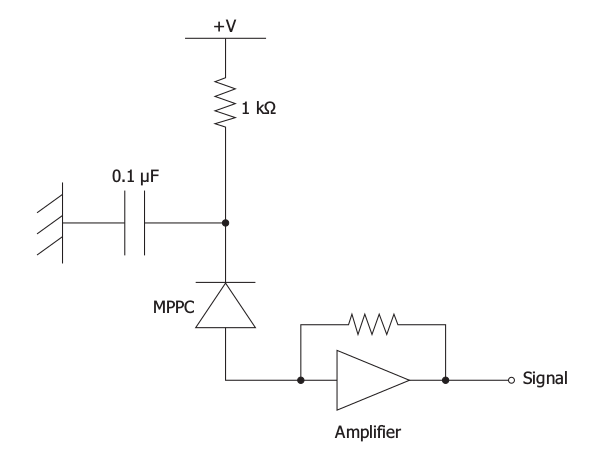
\includegraphics[scale=0.4]{CircuitoTarjeta.png}
\caption{\textbf{Figura 12}.- Circuito de una tarjeta tipo}
\end{figure}


Es una tarjeta del departamento de electrónica, cuyos ingenieros nos han informado que posee una ganancia de $G=100$. Este será el valor que utilizaremos en el análisis posterior para calcular la ganancia de los SiPM.

%Dado que no conocemos su incertidumbre consideraremos este valor como un valor sin error. Esto nos conducirá a obtener una subestimación de la incertidumbre de la ganancia de los SiPM. Sin embargo esto no tiene mayor importancia ya que será un factor constante que afectará por igual a todas las medidas y no estamos buscando determinar la ganancia de los SiPM sino únicamente sus dependencias con el voltaje y la temperatura. 